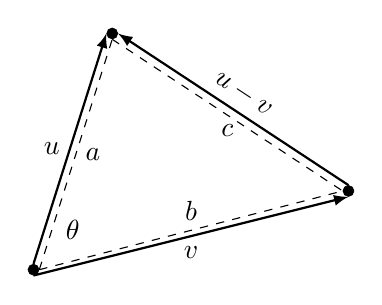
\begin{tikzpicture}[
	point/.style={circle,draw,very thin,fill,inner sep=0pt,minimum size=4pt},
	vector/.style={-latex},
]
	\node[point] at (0,0) (o) {};
	\node[point] at (1,3) (u) {};
	\node[point] at (4,1) (v) {};
	\draw[vector,thick] (o.north) to node[left] {$\uvec{u}$} (u.west);
	\draw[dashed] (o.east) to node[right] {$a$} (u.south);
	\draw[vector,thick] (o.south) to node[below] {$\uvec{v}$} (v.south);
	\draw[dashed] (o.east) to node[above] {$b$} (v.west);
	\draw[vector,thick] (v.north) to node[above,sloped] {$\uvec{u}-\uvec{v}$} (u.east);
	\draw[dashed] (u.south) to node[below] {$c$} (v.west);
	\node at (0.5,0.5) {$\theta$};
\end{tikzpicture}
